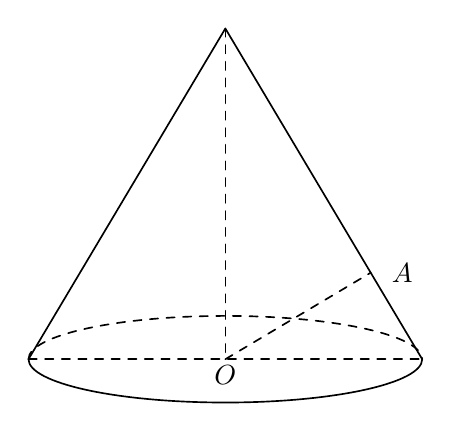
\begin{tikzpicture}[line width=0.6pt, line join=round, line cap=round, font=\normalsize]
  % cone: apex B(top), base center O, base ellipse
  \coordinate (B) at (0,4.2);
  \coordinate (O) at (0,0);
  \coordinate (R) at (2.5,0);
  \coordinate (L) at (-2.5,0);
  \coordinate (A) at (1.8459606530,1.0987861030);
  % axis (dashed)
  \draw[dashed] (B) -- (O);
  % small tick at axis mid (rotation center mark)
  
  % generators solid
  \draw (B) -- (L);
  \draw (B) -- (R);
  % base: front solid, back dashed
  \draw (L) arc [x radius=2.5, y radius=0.55, start angle=180, end angle=360];
  \draw[dashed] (L) arc [x radius=2.5, y radius=0.55, start angle=180, end angle=0];
  % horizontal diameter dashed
  \draw[dashed] (L) -- (R);
  % OA dashed
  \draw[dashed] (O) -- (A);
  % labels with clearance
  \node at (0,-0.20) {$O$};
  \node[right=4pt] at (A) {$A$};
\end{tikzpicture}
